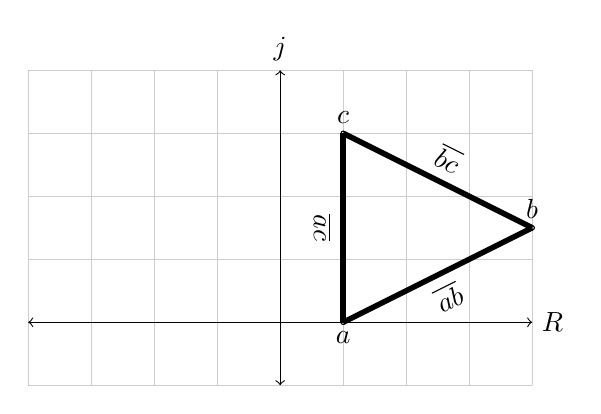
\begin{tikzpicture}[scale=0.8]
    \draw [thin,gray!40] (-4,-1) grid (4,4);
    \draw[<->] (-4,0)--(4,0) node[right] {$R$};
    \draw[<->] (0,-1)--(0,4) node[above]{$j$};
    \coordinate (a) at (1,0);
    \coordinate (b) at (4,1.5);
    \coordinate (c) at (1,3);
   
    \draw[black] (a) circle(1pt) node[anchor=north]{$a$};
    \draw[black] (b) circle(1pt) node[anchor=south]{$b$};
    \draw[black] (c) circle(1pt) node[anchor=south]{$c$};
    \draw[line width=2pt,black,-] (a)--(b) node[midway, below, sloped]{$\overline{ab}$};
    \draw[line width=2pt,black,-] (b)--(c) node[midway, above, sloped]{$\overline{bc}$};
    \draw[line width=2pt,black,-] (c)--(a) node[midway, below, sloped]{$\overline{ac}$};
\end{tikzpicture}
\caption*{Triangulo $s$}